\section{Prestudy}\label{Prestudy} This project is one that requires quite a lot of prestudy before we can begin coding or even designing the architecture. Since the customer wanted us to implement existing technologies, such as Glassfish, WSO2, SAML etc. we needed to spend some time researching those technologies to figure out what to use, and how to use it. The following sections will describe the the overall architecture of how we imagined our system to be like. 

        \begin{figure}[htb]
            \centering
            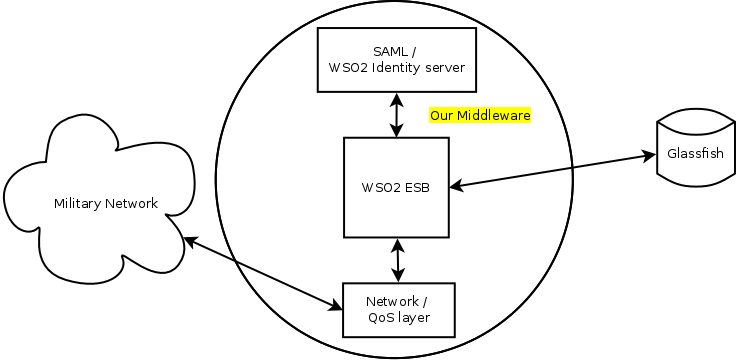
\includegraphics[width=\textwidth]{birdarch}
            \caption{Birds eye view of the overall architecture.}
            Our initial thought of the basic view of our system. 
            \label{fig:birdarch}
        \end{figure}

    \subsection{Server side Architecture}\label{Server side Architecture}
    
        The server side architecture consists of several components, the WSO2 ESB, the WSO2 \gls{identity server}, the Tactical Router and the GlassFish server. All of these components are already available, so what we will have to make is \glspl{mediator}\footnote{\Gls{mediator} - A component in WSO2 ESB which can be used to work on incoming or outgoing messages that passes through the ESB} in the ESB.

        Before the client can request a web service it has to have an identification. To get an ID-\gls{token} it has to contact the Identity Server using the ESB as a \gls{proxy}\footnote{\Gls{proxy} - A proxy server acts as an intermediary between clients and servers} (Fig.\ref{fig:Serversidearchitecture}-1). Then the client can request a web service from the ESB. Several things will then happen in the ESB. First the request message is sent to the SAML mediator (Fig.\ref{fig:Serversidearchitecture}-2), this mediator contacts the Identity Server to validate the clients ID-token (Fig.\ref{fig:Serversidearchitecture}-3). If the token is validated and the client is supposed to have access to the requested service, the message is passed on to the GlassFish proxies (Fig.\ref{fig:Serversidearchitecture}-4), otherwise it is dropped. The ESB acting as a proxy will then send the request along to the requested service on the GlassFish server (Fig.\ref{fig:Serversidearchitecture}-5).

        \begin{figure}[htb]
            \centering
            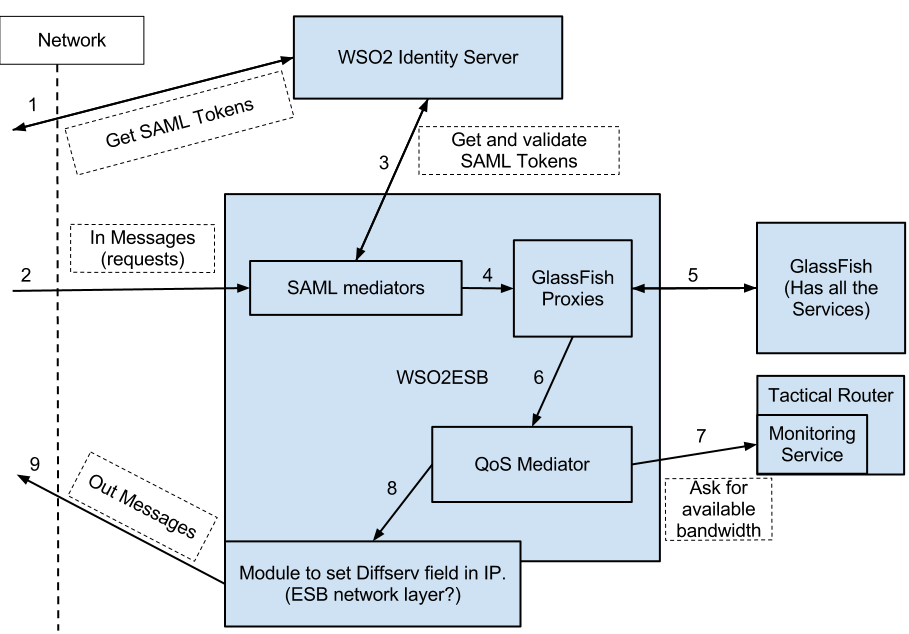
\includegraphics[width=\textwidth]{Serversidearchitecture}
            \caption{The Server side Architecture}
            This is the overall design of our implementation of the server side. It shows the modules in the server and the flow in the system. 
            \label{fig:Serversidearchitecture}
        \end{figure}

        When the request is received at the service, it will probably start sending some data to the client. This is also done through the ESB. First the message is sent to the QoS mediator (Fig.\ref{fig:Serversidearchitecture}-6). This mediator will first look at the role, or identity, of the client and the service requested, and use this information to assign a priority to the connection. Then the \gls{ms}\footnote{Monitoring Service, a service that provides bandwidth monitoring, running on the same server as the Tactical Router} on the Tactical Router is contacted for bandwidth information (Fig.\ref{fig:Serversidearchitecture}-7), which is used together with the priority to determine whether the message should be sent right away or held back until some higher priority message is finished sending.

        Either in the QoS mediator, in the ESB’s network layer, or after that, the Diffserv (ToS) field of the IP header will have to be set (Fig.\ref{fig:Serversidearchitecture}-8) before the message is sent to the client (Fig.\ref{fig:Serversidearchitecture}-9). This field is used by the routers in the network to prioritize packet sending. This step is quite important to the whole procedure as this is one of the few requirements the customer has given us, as such this step can not be dropped from the final product.
 
    \subsection{Client side Architecture}\label{Client side Architecture} 
    
        The client-side architecture will be composed of altered (already existing) client software, the \gls{opensaml}\footnote{\gls{opensaml} - A set of open source C++ and Java libraries to support developers working with SAML. [\url{https://wiki.shibboleth.net/confluence/display/OpenSAML/Home/}]} library as well as our client library implementation.
        
        \begin{figure}[htb]
            \centering
            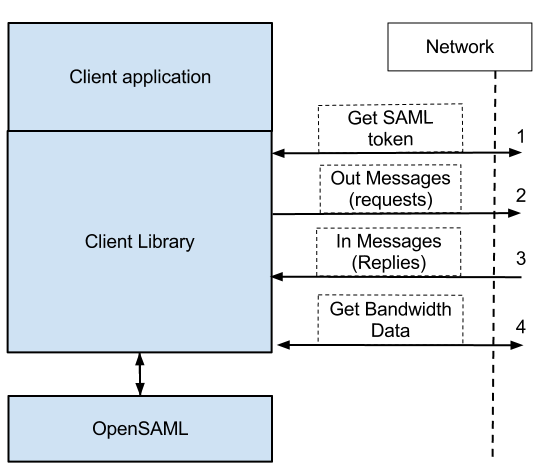
\includegraphics[scale=0.5]{Client-sideArchitechture}
            % do not import the new figure as the old one is corret as this is the prestudy. 
            \caption{The Client side Architecture}
            The client architecture shows the basic thought of how the system should look like and the communication to and from the client library. 
            \label{fig:Client-sideArchitechture}
        \end{figure}
 
        Before the client library can ask for the data the client needs to get a SAML authentication token from the identity server (Fig.\ref{fig:Client-sideArchitechture}-1). The communication here will most likely be handled by our library, but the SAML packages will be created and analyzed by the OpenSAML library. 

        The client library then sends the request from the client to the server (Fig.\ref{fig:Client-sideArchitechture}-2), appending the SAML token to the package as well as adding some metadata in the SOAP header related to the client role and setting the TOS field of the package to a default value.

        The reply from the server is examined by our client library for the metadata the server has embedded in the SOAP header, relevant metadata is stored for future communication and the package is passed to the client application (Fig.\ref{fig:Client-sideArchitechture}-3).

        When new communication is initiated after this first connection is made the client should, if everything went as expected, have the necessary information to prioritize new messages. This means that the client can now take an informed decision about how it should prioritize messages, but in order to do this to the best of it’s abilities it also has to take into consideration available bandwidth (Fig.\ref{fig:Client-sideArchitechture}-4).
    
    \subsection{Unit testing}\label{Unit testing}
    We decided quite early on that we wanted to do unit testing of every piece of code that we would produce, i.e. test driven development. The reason behind this choice is that we think it will result in better code quality. An added bonus is the simplification of integration testing, due to easier discovery of whether a new code addition will integrate with the old code. Also writing the tests first lets us concentrate more on exactly what the methods should do, instead of the content and how it should do it. One of the problems with test driven development however, is the possible bias that could occur, we could end up only satisfying the test and not the actual requirements. This could be countered to some extent by writing more comprehensive tests. Another positive point in favour of unit testing is the requirement we have, which states that the product has to be written in Java where such test are easy to integrate and write using JUnit.

    \subsection{Integration testing}\label{Integration testing}
   For integration testing, we decided that we wanted to do automated system testing every other week in collaboration with code reviews. The procedure we are going to follow will be coding new features in a separate branch. Once every other week the finished branches will have all their unit tests run thoroughly, followed by a code review of at least one person. Then if the automated system tests are fully operational, they will also be run to look for additional errors which the unit tests can not pick up. This point is likely to change in the future as a two week time interval might be to long given the short implementation period. The advantage of doing this integration testing is better overall code quality, since we will test code before it is used by other parts of the system. Since we are also doing code reviews, people will also gain experience with other parts of the system which they previously had not worked on. This will benefit everyone since knowledge about the system is shared, and it will help in the eventuality of someone getting sick. The advantage of developing in separate branches is the reduced risk of polluting code other people are working on, and a better separation of stable and unstable code.

    \subsection{System testing}\label{System testing}
    When it comes to system testing, the customer was quite insistent that we test the product thoroughly in an emulated network situation. Since we have had some experience with NS3 we decided that we wanted to do the system testing on it. The advantage with this, is that the customer has already set up some testing scenarios and helper-scripts designed for NS3, which they offered for our use. This will greatly reduce the time needed for setting up the test suite, and it will also give us the ability to have automated tests, which we don’t have to monitor or interact with. Another added advantage is easy testing, as we only have to start a script in order to run the whole suite, but that comes at the cost of actually setting up the whole thing. As of the midterm report, we have set quite a lot of time aside in order for us to implement the proper NS3 support we need. To monitor what is happening during the test-runs, our applications will output all important information regarding what is going on, in addition to this we will have a \gls{packet sniffer} on each end which will capture network traffic. Using this information we should be able to tell a whole lot about what is going on in the network and we should be able to decide whether we have met the requirements or not.

    Below are some of the detailed test cases which we will automate on top of NS3. The testing itself will be automated, but in order to get some result from the tests, some human interaction is needed to interpret the output data.
\\
    \begin{figure}[h]
        \centering
        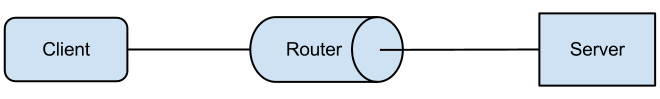
\includegraphics[scale=0.4]{Simplemessagesending}
        \caption{Simple message sending}
        One client communicates with one server through one router.
        \label{fig:Simple message sending}
    \end{figure}
\\
Simple message sending:\\
    In this test, shown in figure \ref{fig:Simple message sending}, we want to test the ability of the client and the ESB to communicate. We want to see that the client is able to send messages(\gls{message}) to the server and get a response back. For monitoring purposes, this test will rely on both applications to log their behavior. In order for us to give this test the green light we must see a message going out from the client then passing through the ESB to GlassFish. Then finally a reply should be sent back from GlassFish to the ESB and then to the client.
\\\\
Setting Quality of Service:\\
    In this test, we want to test the client and the ESB’s ability to set the DiffServ field in the IP header. The first requirement is that the test “Simple message sending” has been passed. For this test to be considered a success, the client has to send a message to the ESB, which is responds with the DiffServ value in the SOAP header. The ESB must at this point have set the DiffServ value in the IP header. The client should then use a service on GlassFish, but this time the IP header must contain the correct DiffServ value. In order to monitor this test, only a packet sniffer located on the client and ESB side needs to be used. The packets must be examined, and the correct DiffServ value must be present in the IP header of all packets, except the first one going out from the client.
\\
    \begin{figure}[h]
        \centering
        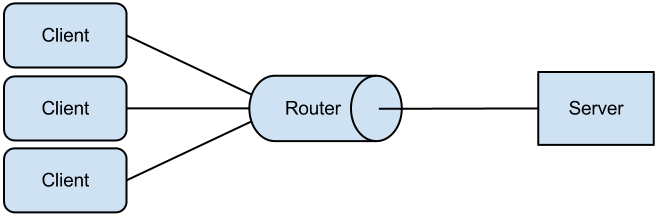
\includegraphics[scale=0.4]{3Clientmessagesending}
        \caption{Three clients message sending}
	Three clients communicate with the same server through the same router. One of the clients will have a higher priority than the two others, in order to test the servers ability to prioritize.
        \label{fig:threeclientmessagesending}
    \end{figure}
\\   
Prioritizing messages:\\
    In this test we want to test the ESB’s ability to prioritize messages. The scenario will be set up as shown in figure \ref{fig:threeclientmessagesending}, with two clients sending lots of messages in an attempt to flood the capacity of the network. All of these messages should have the same priority, but intermittently, a third client with a higher priority will attempt to send some messages. What we are looking for is that these higher priority messages should be sent out from the ESB before the ones with lower priority and, if necessary, it has to stop some already sending messages. For this test to be successful, we must see some lower priority messages being preempted or held back. To do this, the log file of the ESB must be studied, and there should be some clear indications of one of the requirements.
\\\\
Changing DiffServ value:\\
    In this test we want to check the ESB’s ability to change the DiffServ value after a reconfiguration. The test and the result can be performed and examined the same way as “Setting Quality of Service”, but this time the test has to be run twice. One where the configuration has one DiffServ value, and a second run where the DiffServ value has a different value. For the test to be successful, one would have to examine the resulting \gls{pcap}\footnote{\Gls{pcap} is short for Packet capture which in our text this usually refers to a program which captures the traffic on a given socket} files on the server side, and check each run to see if the two tries have different DiffServ values.
\\
    \begin{figure}[h]
        \centering
        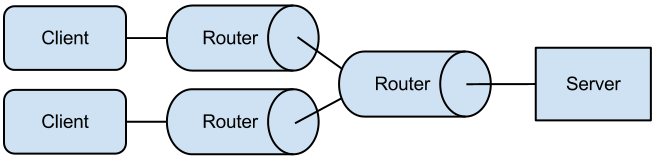
\includegraphics[scale=0.4]{2Clientdifferentpathsmessagesending}
        \caption{Two Clients with different paths}
        Two  clients communicating with the same server, but with different paths.
        \label{fig:2 Clients different paths message sending}
    \end{figure}
\\    
Multipath server routing:\\
    In this test we want to look at the ESB’s capabilities to talk to the MS and understand the routing result. From the MS the ESB should get some routing information about the topology of the network. As you can see in figure \ref{fig:2 Clients different paths message sending}, if the link between the server and the first router is not the limiting factor, the two clients should not get in each others way. Therefore, since we get the information about the last router from the MS, the ESB should understand that there is likely no problem and should not preempt any messages. To check if this is actually the case, the ESB will need some time to adjust as it does not get the full picture of the network topology, but after this time, no messages should be dropped from the ESB’s side.
\\
    \begin{figure}[h]
        \centering
        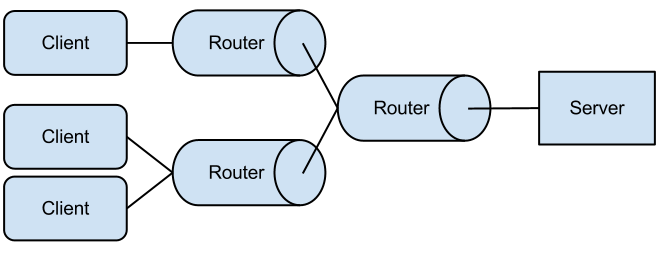
\includegraphics[scale=0.4]{3Clientswheretwoarecompeting}
        \caption{Tree Clients where two are competing}
        Three clients communicate with the same server, but only two of them share the path.
        \label{fig:3clientstwocompeting}
    \end{figure}
\\
Competing clients in a multipath environment:\\
    This test is a compilation of the tests “Multipath server routing” and “Prioritizing messages”. For this test we want to make sure that the ESB is smart enough to only preempt the messages going to one of the competing clients. As you can see in figure \ref{fig:3clientstwocompeting}, there is one client which should not affect either of the two others if the link between the server and the first router is not a bottleneck. This should allow this client to receive messages even though the two other clients are competing for scarce resources. To check that this test is successful, a combination of the clients log files and the server log files will have to be used. If most(over 96\%) of the messages arrive at the higher priority client and the third client is not affected then this test is successful.
\\\\
Competing clients in a low bandwidth scenario:\\
    In this test we want to test that the ESB can manage to prioritize messages in a network with a joint bottleneck, but with different endpoints. In figure \ref{fig:3clientstwocompeting}, if the link between the server and the first router is the bottleneck, the ESB should after a small initialisation understand that it has to preempt messages going out to all clients, in order to let a higher priority client get the service it is supposed to get. The scenario will be set up in such a way that one of the two competing clients will have higher priority than the two others, the two lower priority clients should then send a steady stream of messages, which should fill the bottleneck link. The third client should then start sending some messages which must now fill the entire bottleneck link, and create a situation where the ESB has to hold back or preempt messages going to either of the two other clients. As before, a combination of the ESB and the clients log files have to be examined.
           
    \subsection{Alternative solutions}\label{Alternative solutions}

        The customer also gave us a paper\cite{soa-qos-pdf} which described a previous project they had worked on which tried to solve something quite similar to what we were tasked with. The paper described a system which were used in conjunction with Tactical routers to retrieve bandwidth information and to control sending of messages into this network. As the customer explained this work was not something we could directly copy as the project had not used a lot of web standards and had focused more on the tactical routers as opposed to web services. What we could take out of it however was how they throttled messages. The paper contained five methods which we could easily implement and use their result as an indication of what methods we should use to throttle or hold back messages.

        One architecture, which our customer suggested for the project, was to have a proxy in between nodes and creating a custom QoS layer which would sit in front of both the client and the services. This layer would then communicate with a SAML server for authentication, and would have to do all the message prioritization based on the same criteria as our architecture. There are several points about this architecture which would make it a good fit for us. Since the QoS layer would be identical on both client and server side it would mean less work, and more code that could be shared among components, but this freedom comes with some downsides. The first and most glaring problem encountered would be that services on the server would have to be altered to be able to communicate with this front end. Even though we were free to choose architecture ourselves, the client expressed a wish that we would not choose this model because the customer wants to use \gls{cots}\footnote{\gls{cots} - Commercially available Off-The-Shelf} services which would not be compatible with the new front end.

        Even though the above mentioned architecture is not the best fit for us we wanted to take some aspects of the architecture further. Since clients can easily be altered, the above mentioned solution is not applicable for server side, the solution could however be used for the clients. Having a proxy on the client side could be quite good, but because of the work involved and probable time constraints we chose not to go with this solution. On the server side however a front end is not the best solution for us. What we instead are looking into, is to use an ESB which would be configured together with the services and work as a proxy. Because many ESBs have integrated SAML processing we could easily take advantage of such facilities along with custom message processing, with which we would then extend the ESB to support our needs. The clients would have to point to the ESB, but this should both be trivial to do and the customer has expressed their agreement that this is satisfactory. We could eventually expand the functionality with service discovery, which then would be a good solution to the problem.

        So far we have outlined major alternative architectures which could be alternatives to our project, but there are also alternatives within our proposed solution. One such alternative is not to use a premade ESB, but rather build one ourselves. This solution was thoroughly investigated, but was eventually turned down because of the massive amount of work that had to be done, the quality of an already made ESB is much higher than we could ever achieve during this project, and lastly, the open source tools available to implement the functionality needed for SAML was not very well documented, and would take considerable time to get familiar with.

        On the client side we also have the choice of having either a \gls{http}\footnote{Hypertext Transfer Protocol} proxy or writing our own custom library. Both have some advantages and disadvantages, a proxy would be better for integration with client programs, but creating this proxy or configuring and customizing an already existing solution is not trivial. On the same note, creating a library for use in client programs is easier, but this would mean that client programs would need to be altered to be usable with our middleware, which isn’t that desirable. We chose to go down the road of least resistance, as we see it currently we would have do quite a lot of research into proxies which could in the worst case scenario result in just wasted time as far as our product goes. A client library would from our perspective be easier as we would have more control, the overall design should be easier and we know that with this sort of library we can integrate OpenSAML which is a huge advantage.  
    
    \subsection{Process model}\label{Process model}
    Our initial thoughts on the process was way of. At first we thought we could use scrum methodically and have weekly sprints. And most importantly start coding at once. This was before we really figured out what our task was. And the implications the task had on our approach to a solution. 
    
    When the Task Description and Requirements(\ref{Task Description and Requirements}) became apparent we had to radically rethink our approach to the whole development approach and process. 
    
    The task required us to research a lot before we could design our system. And the design was essential for us to be able to implement a solution to the given task. We ended up with a waterfall like approach. Our project life cycle is described in section \ref{Software project life cycle}.
    
    % TODO: ref gantt chart. 
    The gantt [TODO: ref the gantt chart\ref{The gant chart}] chart is the result of the process planning. In short terms the plan consists of four parts: research, design, implementation, documentation. In practice we found out how to solve the task before we design our final solution. Then we coded and set up the system and tested it. And summarised it all in the documentation part.
    
    \subsection{Tools}\label{Tools}          
          
